%%%%%%%%%%%%%%%%%%%%%%%%%%%%%%%%%%%%%%%%%
% Jacobs Landscape Poster
% LaTeX Template
% Version 1.1 (14/06/14)
%
% Created by:
% Computational Physics and Biophysics Group, Jacobs University
% https://teamwork.jacobs-university.de:8443/confluence/display/CoPandBiG/LaTeX+Poster
%
% Further modified by:
% Nathaniel Johnston (nathaniel@njohnston.ca)
%
% This template has been downloaded from:
% http://www.LaTeXTemplates.com
%
% License:
% CC BY-NC-SA 3.0 (http://creativecommons.org/licenses/by-nc-sa/3.0/)
%
%%%%%%%%%%%%%%%%%%%%%%%%%%%%%%%%%%%%%%%%%

%----------------------------------------------------------------------------------------
%	PACKAGES AND OTHER DOCUMENT CONFIGURATIONS
%----------------------------------------------------------------------------------------

\documentclass[final]{beamer}

\usepackage[scale=1.05, orientation=landscape, size=custom, height=90, width=230]{beamerposter} % Use the beamerposter package for laying out the poster
\usepackage{mathtools}

\usetheme{confposter} % Use the confposter theme supplied with this template

\setbeamercolor{block title}{fg=ngreen,bg=white} % Colors of the block titles
\setbeamercolor{block body}{fg=black,bg=white} % Colors of the body of blocks
\setbeamercolor{block alerted title}{fg=white,bg=dblue!70} % Colors of the highlighted block titles
\setbeamercolor{block alerted body}{fg=black,bg=dblue!10} % Colors of the body of highlighted blocks
% Many more colors are available for use in beamerthemeconfposter.sty

%-----------------------------------------------------------
% Define the column widths and overall poster size
% To set effective sepwid, onecolwid and twocolwid values, first choose how many columns you want and how much separation you want between columns
% In this template, the separation width chosen is 0.024 of the paper width and a 4-column layout
% onecolwid should therefore be (1-(# of columns+1)*sepwid)/# of columns e.g. (1-(3+1)*0.024)/3 = 0.30
% Set twocolwid to be (2*onecolwid)+sepwid = 0.624
% Set threecolwid to be (3*onecolwid)+2*sepwid = 0.9

\newlength{\sepwid}
\newlength{\onecolwid}
\newlength{\twocolwid}
\newlength{\threecolwid}
\newlength{\fourcolwid}
\newlength{\fivecolwid}
\setlength{\paperwidth}{230cm} % A0 width: 46.8in
\setlength{\paperheight}{90cm} % A0 height: 33.1in
\setlength{\sepwid}{0.008\paperwidth} % Separation width (white space) between columns
\setlength{\onecolwid}{0.155\paperwidth} % Width of one column
\setlength{\twocolwid}{0.384\paperwidth} % Width of two columns
\setlength{\threecolwid}{0.588\paperwidth} % Width of three columns
\setlength{\fourcolwid}{0.792\paperwidth} % Width of four columns
\setlength{\fivecolwid}{0.996\paperwidth} % Width of five columns
\setlength{\topmargin}{-0.5in} % Reduce the top margin size
%-----------------------------------------------------------

\usepackage{graphicx}  % Required for including images
\usepackage{booktabs} % Top and bottom rules for tables

%----------------------------------------------------------------------------------------
%	TITLE SECTION
%----------------------------------------------------------------------------------------

\title{Modelling GCaMP responses: From spikes to fluorescence} % Poster title

\author{Thomas J. Delaney$^1$, Michael C. Ashby$^2$, Cian O'Donnell$^1$} % Author(s)

\institute{$^1$Department of Computer Science, $^2$School of Physiology, Pharmacology and Neuroscience, University of Bristol, UK} % Institution(s)

%----------------------------------------------------------------------------------------

\begin{document}

\addtobeamertemplate{block end}{}{\vspace*{2ex}} % White space under blocks
\addtobeamertemplate{block alerted end}{}{\vspace*{2ex}} % White space under highlighted (alert) blocks

\setlength{\belowcaptionskip}{2ex} % White space under figures
\setlength\belowdisplayshortskip{2ex} % White space under equations

\begin{frame}[t] % The whole poster is enclosed in one beamer frame

\begin{columns}[t] % The whole poster consists of three major columns, the second of which is split into two columns twice - the [t] option aligns each column's content to the top

\begin{column}{\sepwid}\end{column} % Empty spacer column

\begin{column}{\onecolwid} % The first column

%----------------------------------------------------------------------------------------
%	INTRODUCTION
%----------------------------------------------------------------------------------------

\begin{block}{Introduction}

The use of fluorescent calcium indicators, such as GCaMP6s to monitor neuronal activity is widespread. But the relationship between GCaMP6s fluorescence and action potential firing is poorly understood.

\hspace{2cm} Furthermore, the effects of the indicator characteristics on this fluorescence signal are unknown. For example, it is known that the GCaMP6s indicator accumulates within neurons over weeks and months, which creates difficulties in comparing activity statistics across time-points. As a result, whether or not spike train inference is always possible using GCaMP6s fluorescence remains unknown.

\end{block}

\begin{figure}
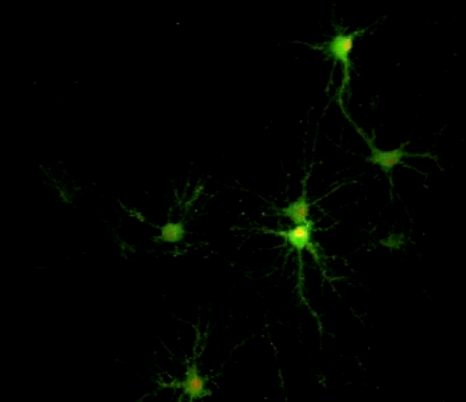
\includegraphics[width=0.7\linewidth]{GCaMP6_fluorescence.png}
\caption{Single frame from video of spontaneous activity recorded from cultured mouse hippocampal neurons using GCaMP6s fluorescent indicator. Image courtesy of  brainslicemethods.com}
\end{figure}

\begin{block}{Aims}

\begin{enumerate}
	\item To simulate the fluorescence traces produced by a fluorescent calcium indicator in a neuron soma.
	\item To understand how indicator characteristics affect fluorescence signal-to-noise ratio and the quality of spike train inference.
	\item To facilitate benchmarking of the various spike inference algorithms that have recently been developed.
\end{enumerate}

\begin{figure}
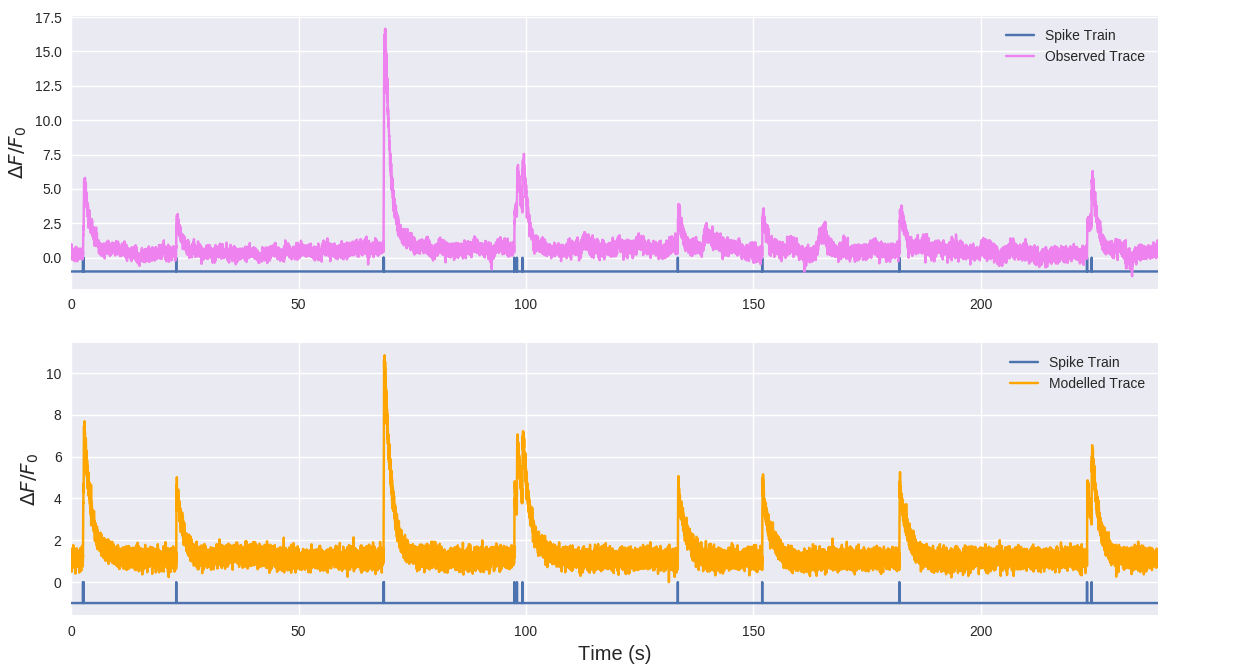
\includegraphics[width=0.8\linewidth]{Observed_vs_Modelled_Fluorescence.png}
\caption{The violet trace is the observed fluorescence from the primary visual cortex in an anesthetized mouse watching a drifting grating movie. The spike train was measured simultaneously using electrophysiological methods.

The orange trace is produced by the fluorescent indicator model after parameter calibration.}
\end{figure}

\end{block}

\end{column} % End of the first column

%----------------------------------------------------------------------------------------

\begin{column}{\sepwid}\end{column} % Empty spacer column

\begin{column}{\onecolwid}

%----------------------------------------------------------------------------------------
%	Methods
%----------------------------------------------------------------------------------------

\begin{block}{Methods}

\begin{itemize}
	\item We modelled five dynamic variables, the concentrations of:
		\begin{description}
			\item[\hspace{2cm}Free calcium ions,]
			\item[\hspace{2cm}Fluorescent indicator proteins,]
			\item[\hspace{2cm}Mobile endogeneous buffers,]
			\item[\hspace{2cm}Immobile endogeneous buffers,]
			\item[\hspace{2cm}Excited indicator bound calcium molecules.]
		\end{description}
		These were modelled using a system of first order ODEs. The equations modelled reactions similar to that of the fluorescent indicator and calcium reactions described above, except without the photon dynamics.
	\item Action potentials were modelled by an instantaneous jump in the concentration of free calcium ions.
	\item Collecting the released photons was modelled as a random variable with binomial distribution.
\end{itemize}

% \begin{figure}
% 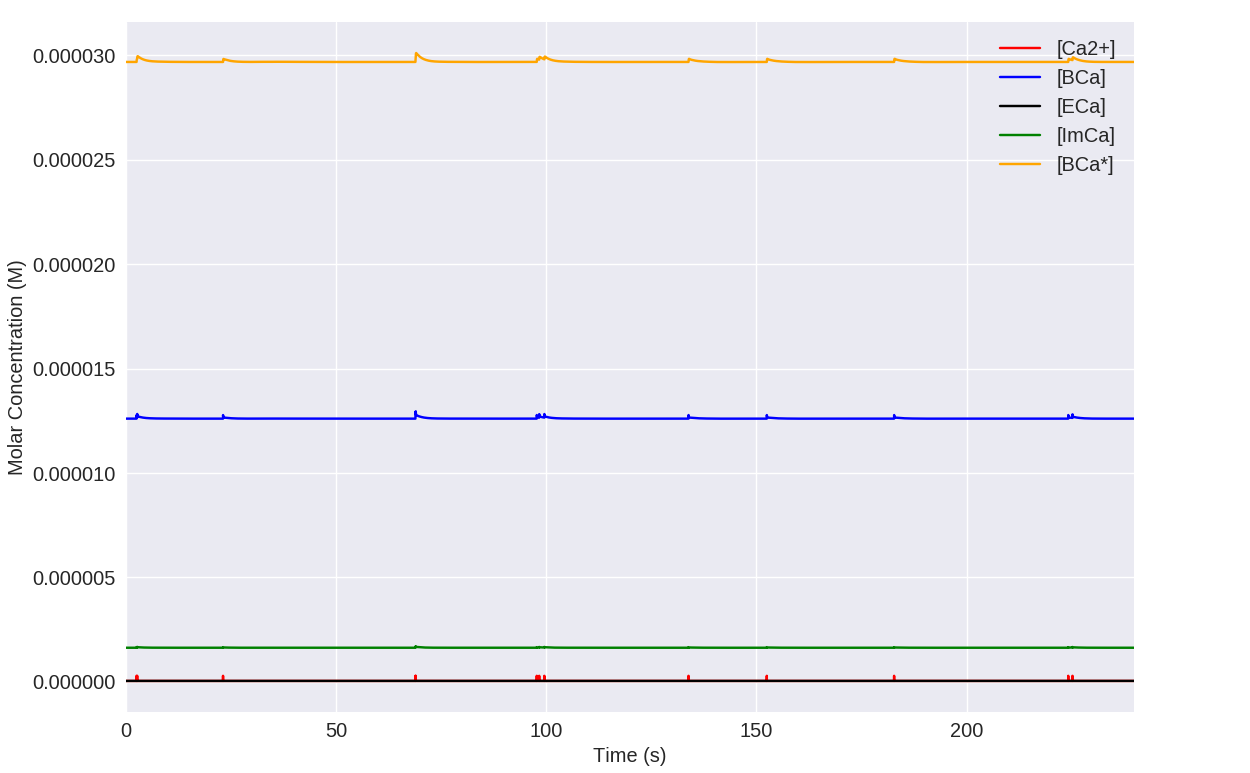
\includegraphics[width=0.75\linewidth]{Full_dynamics_of_model.png}
% \caption{The dynamics of the concentrations. Concentrations of free calcium, bound fluorescent indicator molecules, and bound mobile and immobile endogenous calcium buffers were modelled.
%
% Below are zoomed versions of the figure above, showing the dynamics of each of the concentrations around the time of the action potential at 23s. The indicator and endogeneous buffer bound calcium concentrations decay in two stages, one fast decay, and one slow decay. The excited indicator bound calcium concentration has a rapid increase followed by a slow decay.}
% \end{figure}

\begin{figure}
	\centering
	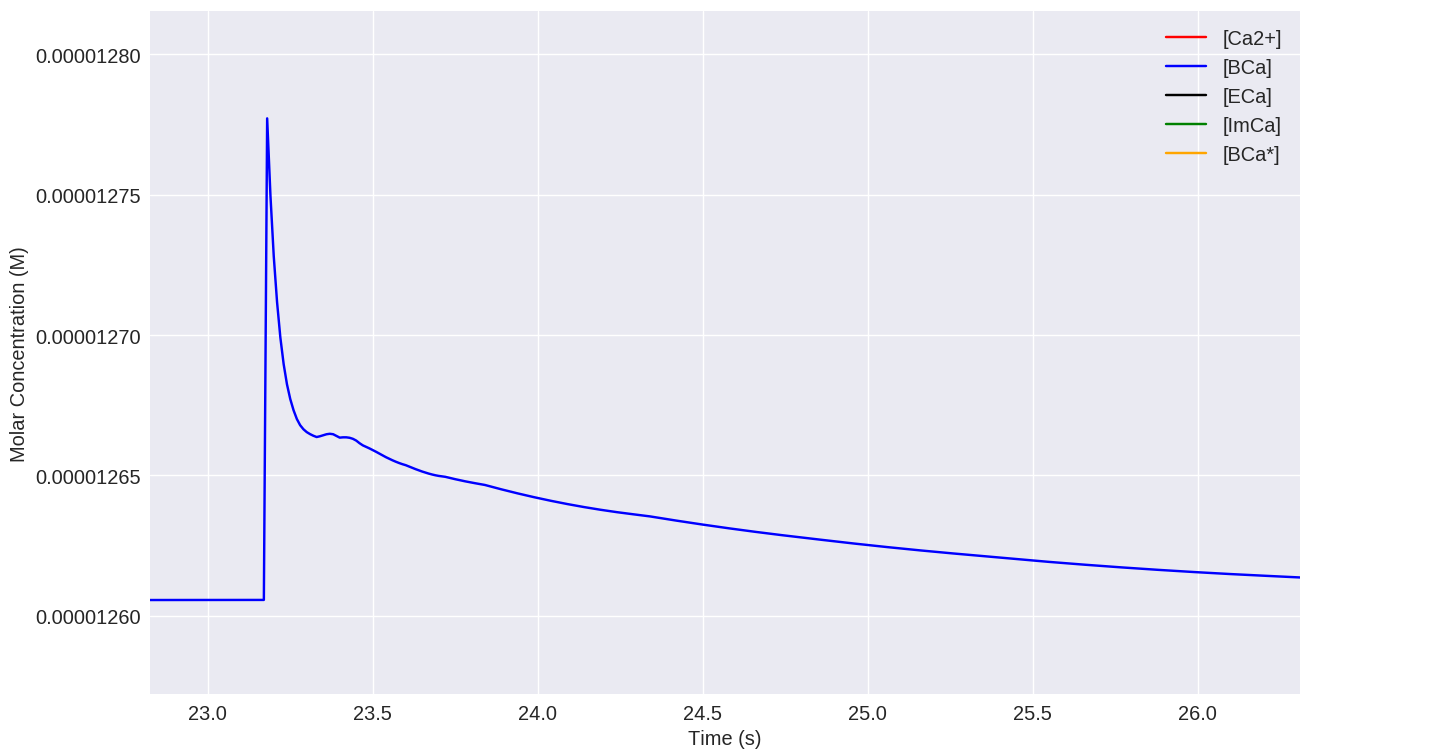
\includegraphics[width=0.48\textwidth]{concentration_dynamics_18_zoomed_BCa.png}
	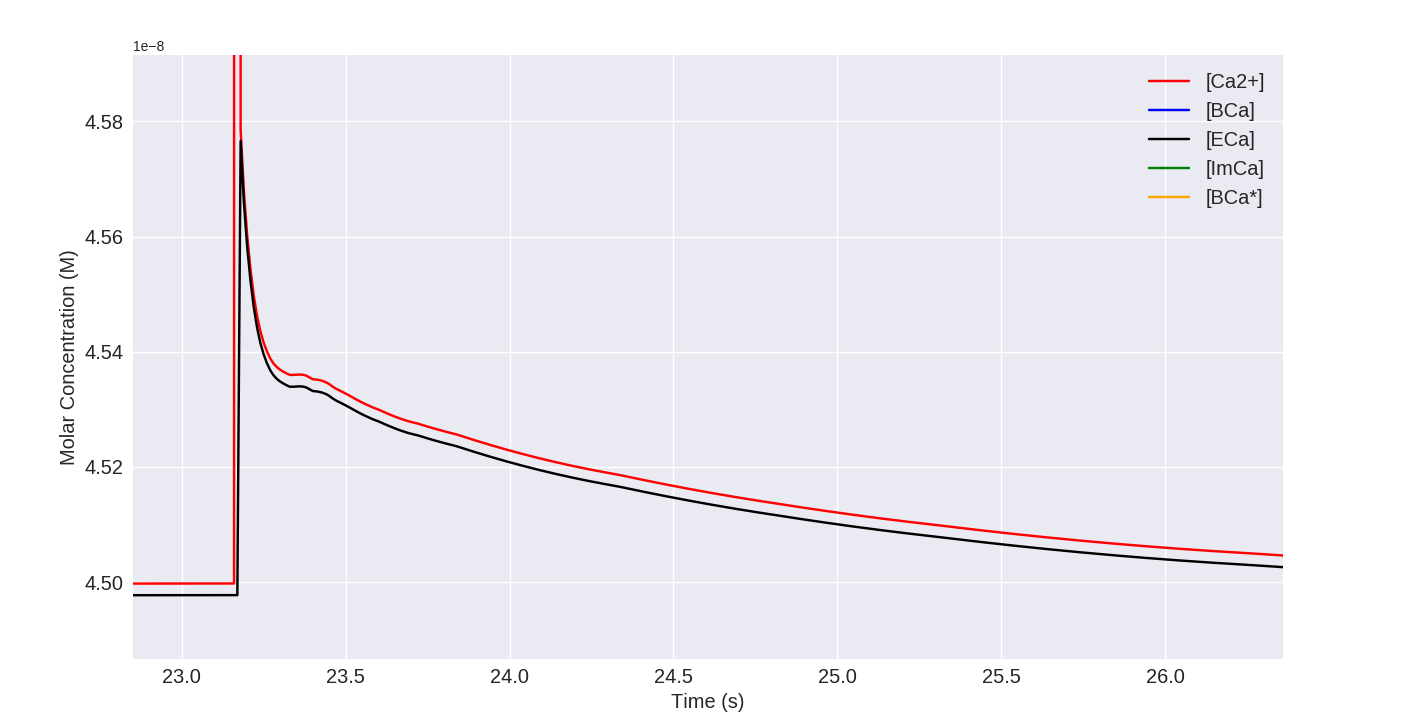
\includegraphics[width=0.48\textwidth]{concentration_dynamics_18_zoomed_ECa.png} \\
	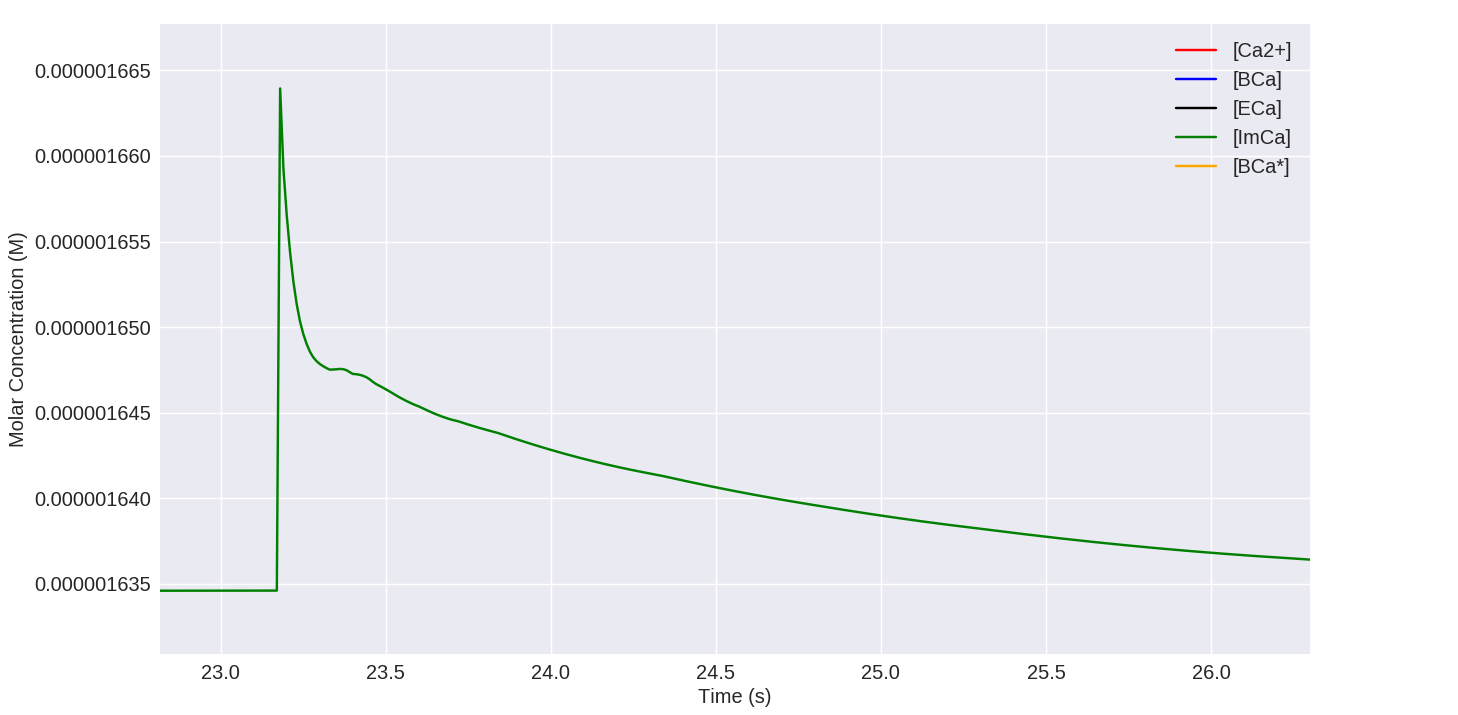
\includegraphics[width=0.48\textwidth]{concentration_dynamics_18_zoomed_ImCa.png}
	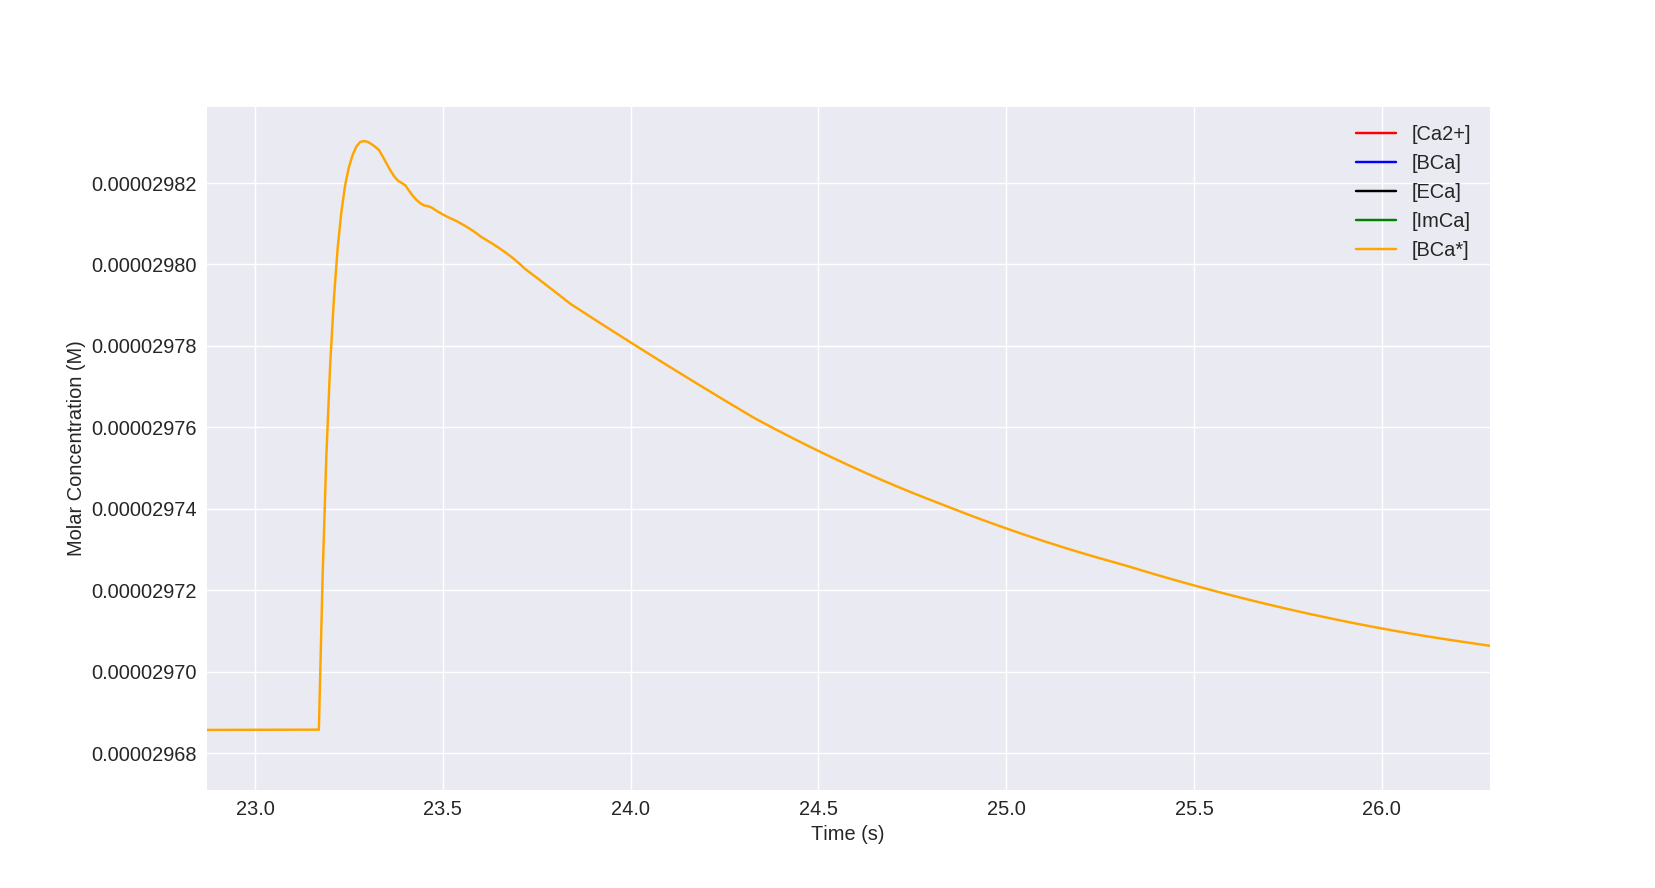
\includegraphics[width=0.48\textwidth]{concentration_dynamics_18_zoomed_excited.png}
	\caption{Dynamics of indicator bound calcium concentration [BCa], endogeneous mobile bound calcium concentration [ECa], endogeneous immobile bound calcium concentration [ImCa], and excited indicator bound calcium concentration around one action potential (top left, top right, bottom left, bottom right respectively).}
\end{figure}

\begin{alertblock}{Two-photon imaging with fluorescent calcium indicators}

When an action potential is fired by a neuron, the concentration of free calcium [Ca$^{2+}$] within the neuron increases rapidly, and decays relatively slowly. These calcium ions bind to proteins within the neuron cytoplasm called \textit{buffers} [B]. The fluorescent indicator is another one of these buffers, with the special property that the indicator bound calcium molecules can fluoresce (release a photon).

%\vspace{1cm}
\begin{center}
	\begin{tabular}{ccccc}
		[B][Ca$^{2+}$] & $\xrightleftharpoons[b]{f}$ &  [BCa] & $\leftrightsquigarrow$ & [BCa$^*$]
	\end{tabular}
\end{center}
%\vspace{1cm}

In two-photon imaging, fluorescent indicator is inserted into a piece of brain tissue either by injection, transportation by a virus, or expression from genetically modified neurons. Photons are then fired at the target piece of tissue. If one of the indicator bound calcium molecules [BCa] is excited by these photons, the molecule will release another photon in turn. The photons released by the [BCa] molecules can then be used to form an image of the tissue showing the neurons.
\end{alertblock}

% \begin{figure}
% 
\includegraphics[width=0.4\linewidth]{Julia_language.png}
% %\caption{Figure caption}
% \end{figure}

\end{block}

\end{column} % End of column 2

%% THIRD COLUMN

\begin{column}{\sepwid}\end{column} % Empty spacer column

\begin{column}{\onecolwid} % The third column

\begin{block}{Fitting Free Parameters}

Our model of the calcium and fluorescence dynamics has four free parameters:

\begin{description}
	\item[Calcium rate, $\beta$] This is the rate at which the [Ca$^{2+}$] concentration is driven back to the baseline \cite{maravall} concentration level.
	\item[Excitation rate, $e$] This defines how many indicator bound calcium molecules become excited by photon bombardment per second.
	\item[Release rate, $r$] This defines how many excited indicator bound calcium molecules will release a photon and go back to their relaxed state per second.
	\item[Capture rate, $p$] This defines the probability of a photon detector capturing a photon released by an excited indicator bound calcium molecule. It is essentially the $p$ parameter of the binomial distribution used to model the photon capture process.
\end{description}

The optimal values for the free parameters were found using a suite of stochastic optimisation algorithms. The objective function was the sum of the root-mean-squared difference between the observed fluorescence trace and the modelled fluorescence trace and the root-mean-squared difference between the smoothed power spectra of the observed fluorescence trace and the modelled fluorescence trace. The lower the value of the objective function, the better the optimisation.

\vspace{5mm}
\begin{figure}
	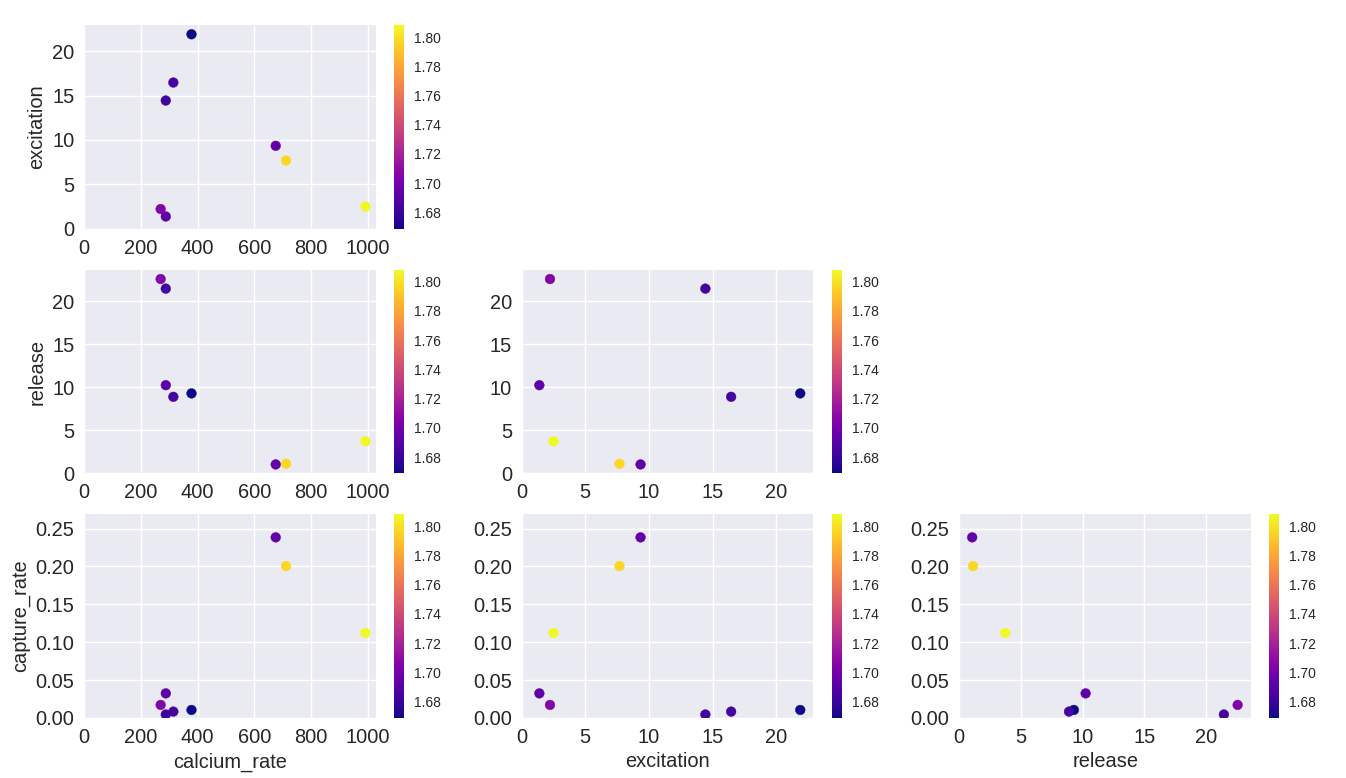
\includegraphics[width=\linewidth]{opcc_18.png}
	\caption{Relationships between optimised free parameters for a given trace. Each data point corresponds to a set of optimised free parameters from one of the seven optimisation algorithms that were applied to the traces. The deep blue points are the better optimised points, the worse optimisations are in yellow.}
\end{figure}
\end{block}

\begin{figure}
	\centering
	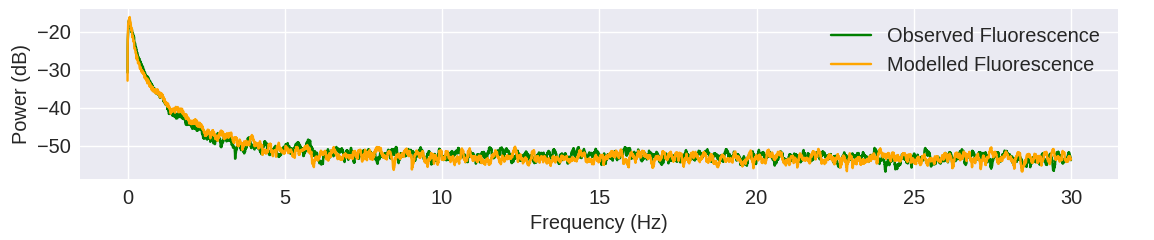
\includegraphics[width=\linewidth]{power_spectrum_comparison.png}
	\caption{The log power spectrum of an observed fluorescence trace, and a modelled fluorescence trace after the fitting procedure.}
\end{figure}

\begin{figure}
	\centering
	
\includegraphics[width=0.2\linewidth]{Julia_language.png}
\end{figure}

\end{column} % End of the third column

\begin{column}{\sepwid}\end{column} % Empty spacer column

\begin{column}{\onecolwid} % The fourth column

\begin{block}{Perturbing parameters}

\begin{itemize}
	\item We varied the parameters of the model and created fluorescence traces.
	\item We measured the signal-to-noise ratio of the traces, using the perturbed and experimental values. We used the ratio of the mean $\Delta F/ F_0$ to the mean noise $\sigma$ in the fluorescence trace as the definition of the SNR.
	\item Then we used a deconvolution algorithm \cite{pnevmatikakis} to infer spike trains from these traces. We measured the quality of the inference using the \textit{true-positive rate}, aka. the \textit{recall} or \textit{hit-rate}.
\end{itemize}

\end{block}

\begin{block}{Varying the fluorescent calcium indicator concentration}

We perturbed the concentration of the fluorescent calcium indicator within the cell soma around the experimental value in order to assess the effect on fluorescence. We used four perturbed values, two higher and two lower.

\hspace{2cm} The higher and lower perturbations affected the fluorescence traces in different ways. But for the more extreme perturbations, the SNR ratio decreased and the inference quality decreased either way.

\vspace{1cm}
\begin{figure}
	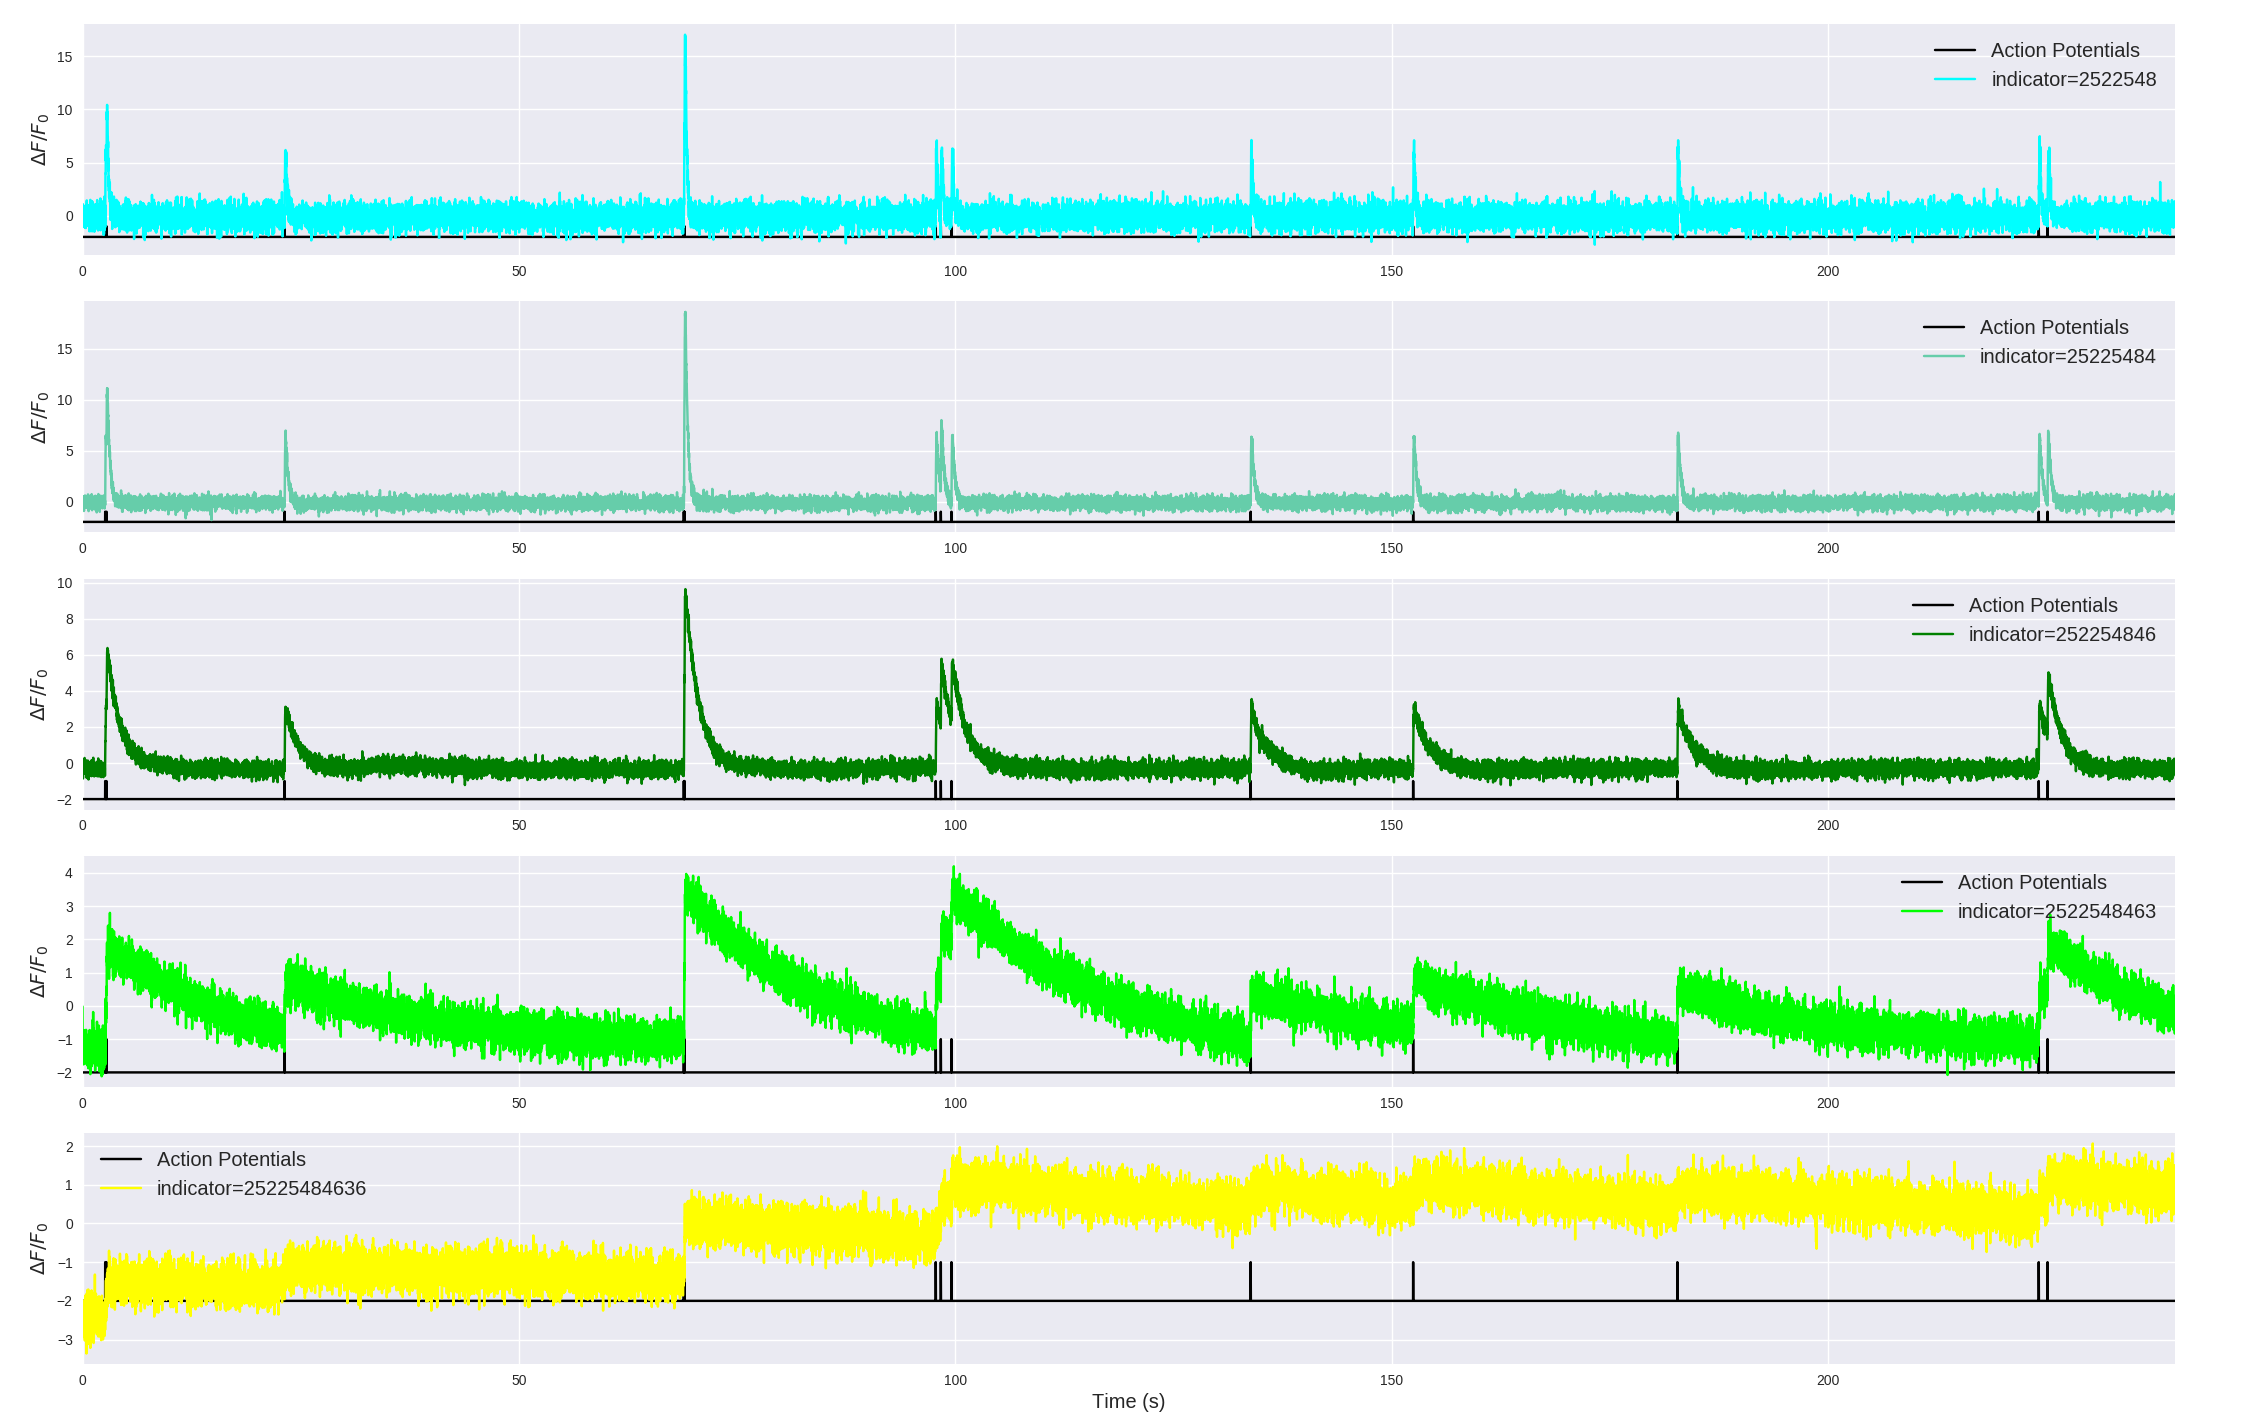
\includegraphics[width=0.33\linewidth]{indicator_peturbed_fluorescence_18.png}
	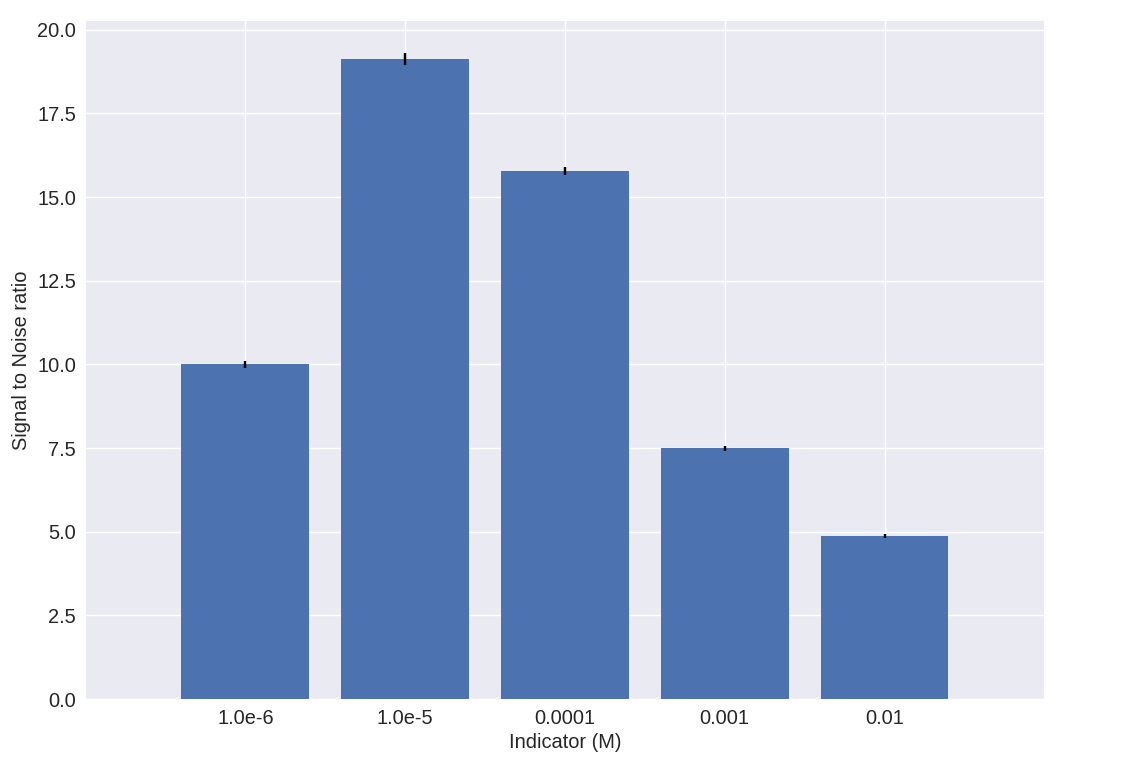
\includegraphics[width=0.33\linewidth]{indicator_perturbed_snr.png}
	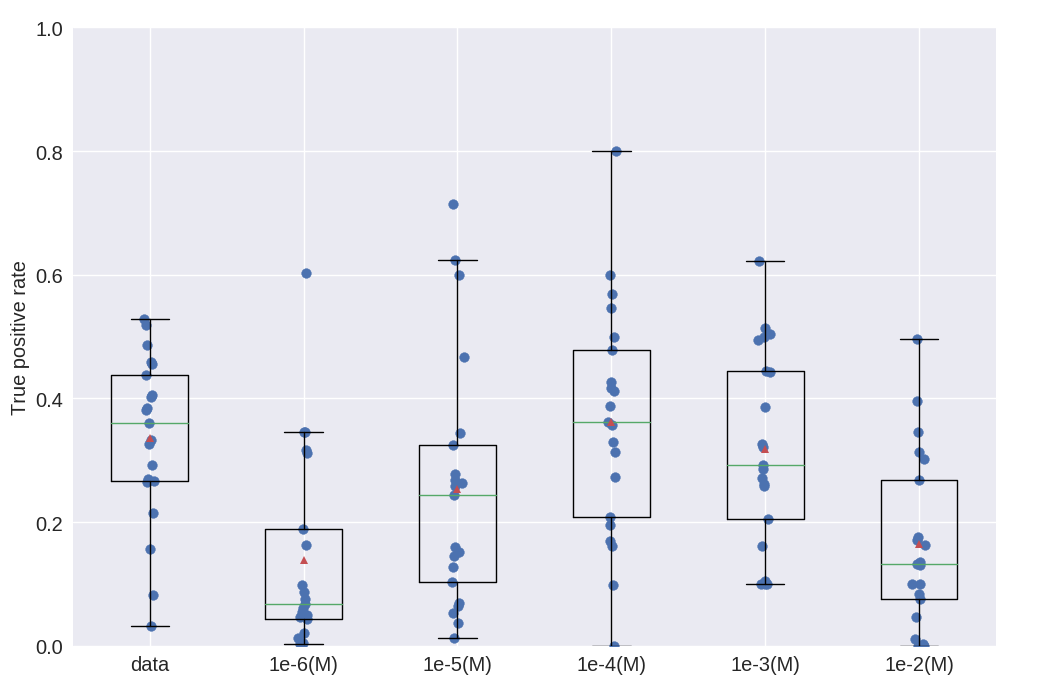
\includegraphics[width=0.33\linewidth]{indicator_perturbed_oasis_first_tp.png}
	\caption{(left) An example trace for each of the five perturbed values for the concentration of fluorescent calcium indicator. The top two traces are produced by the lower perturbed values, the middle trace is produced by the experimental value, and the lowest two traces are produced when using the higher perturbed values.

	(middle) The signal-to-noise ratio of the modelled fluorescence traces using each of the four perturbed values, and the experimental value. Extreme perturbations of the concentration either above or below the experimental level lowered the SNR.

	(right) The true-positive rates of the deconvolution algorithm's predictions when inferring from the observed data, and inferring from modelled traces using the perturbed and experimental values. We found that the algorithms performs equally badly on the two most extreme values, and performs equally well on the experimental value, and the next higher perturbed value.}
\end{figure}

\end{block}

\begin{block}{Varying the immobile endogeneous buffer concentration}

We perturbed the concentration of the immobile endogeneous buffer around the experimental value in order to asses the effects of different levels of immobile buffer on the fluorescence traces.

\hspace{2cm} Having less immobile endogeneous buffer had little effect. But having more immobile buffer caused a smaller change in fluorescence due to an action potential, and a slower decay in fluorescence. The signal-to-noise ratio was also smaller for higher values of immobile buffer as a result.

\end{block}
\end{column} % End of the fourth column

\begin{column}{\sepwid}\end{column} % Empty spacer column

\begin{column}{\onecolwid} % The five column

\begin{block}{Varying the immobile endogeneous buffer concentration}

\begin{figure}
	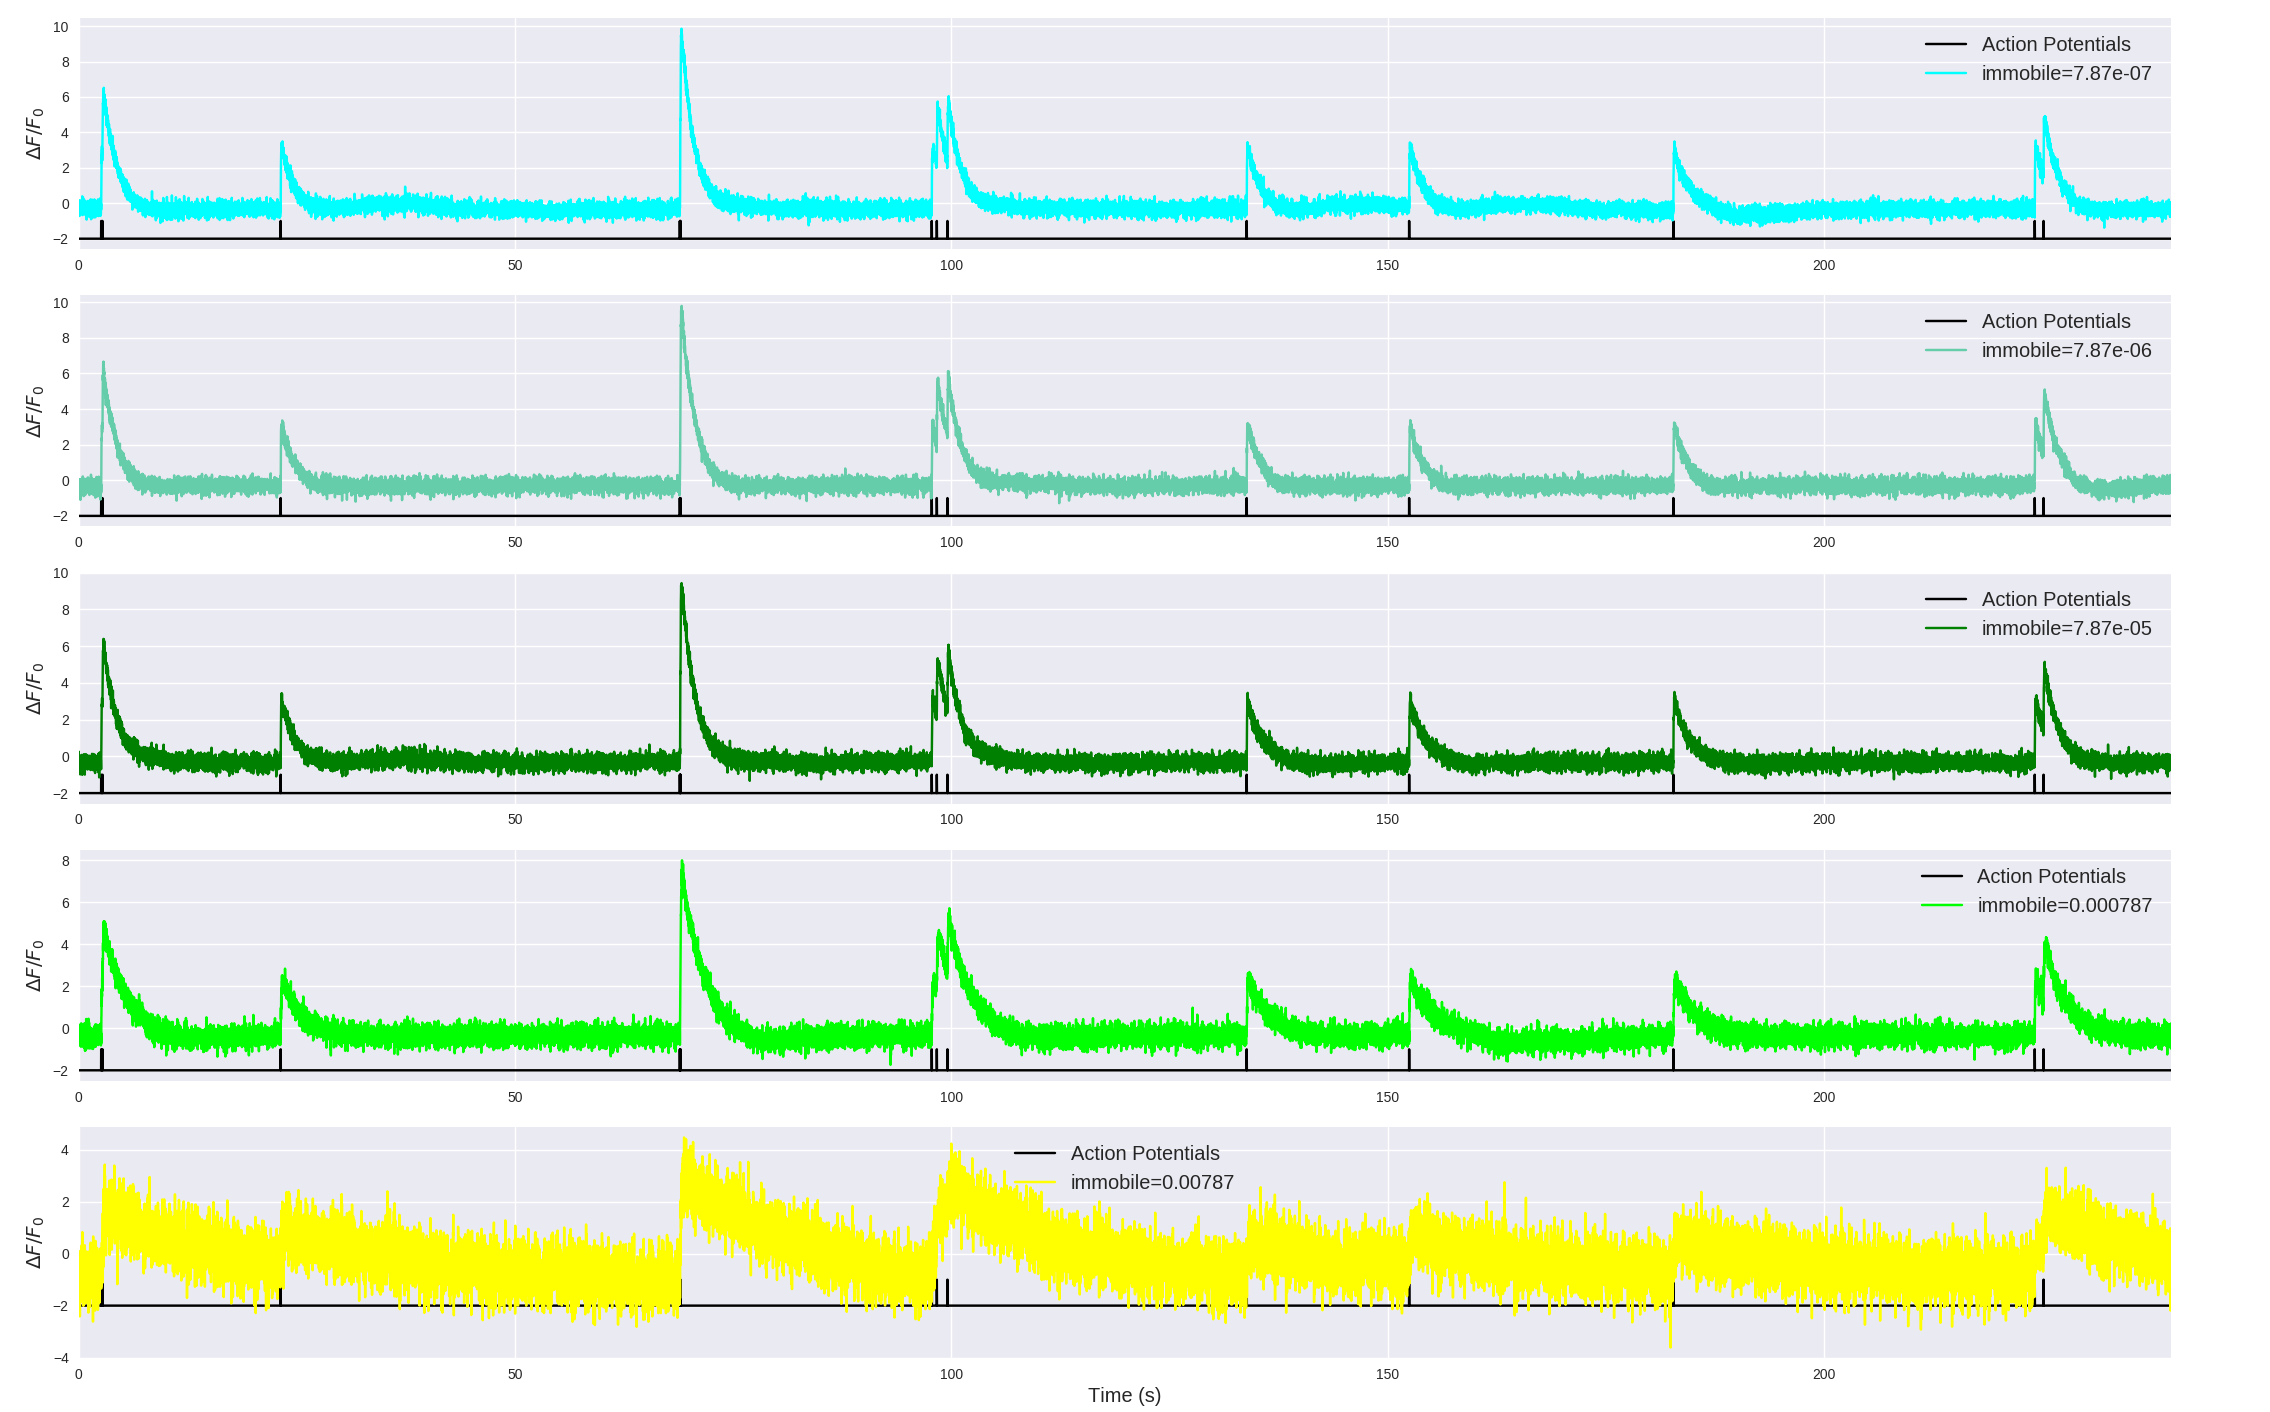
\includegraphics[width=0.33\linewidth]{immobile_peturbed_fluorescence_18.png}
	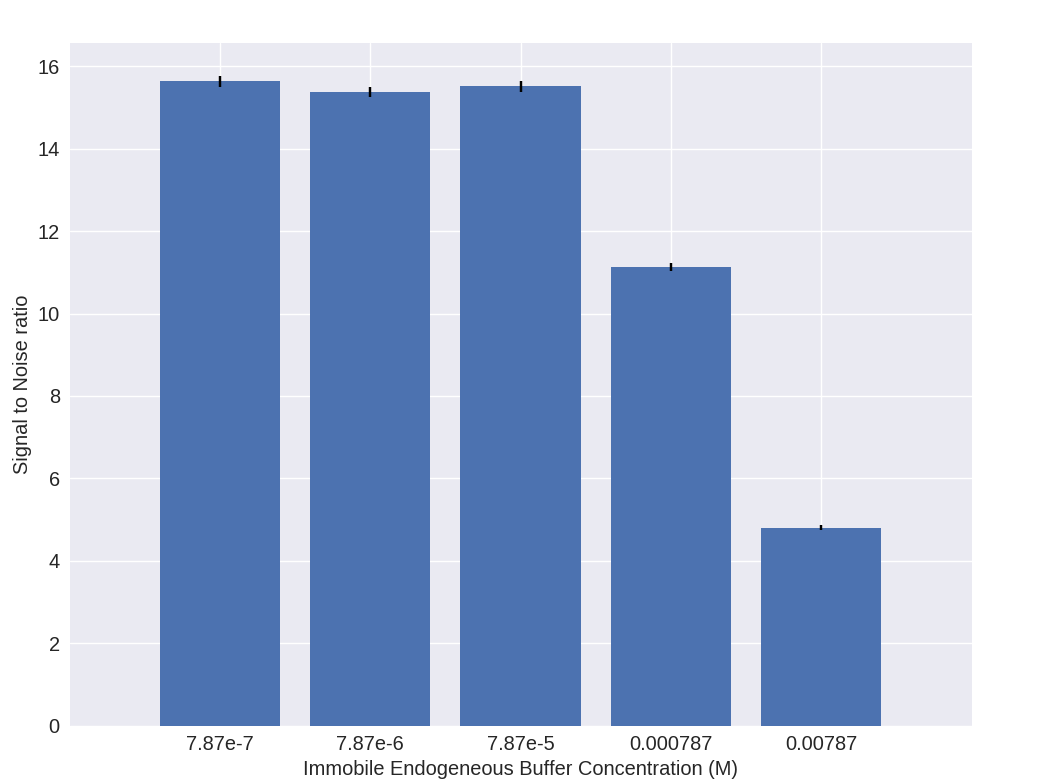
\includegraphics[width=0.33\linewidth]{immobile_perturbed_snr.png}
	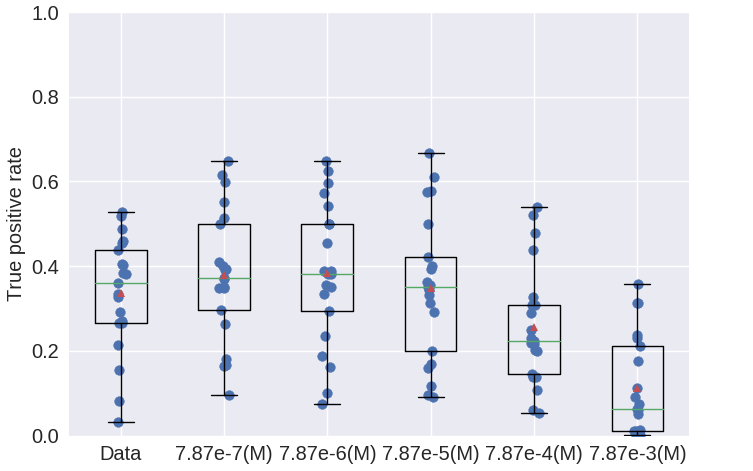
\includegraphics[width=0.33\linewidth]{immobile_perturbed_oasis_first_tp.png}
	\caption{(left) An example trace for each of the five perturbed values for the concentration of immobile endogeneous buffer.

	(middle) The signal-to-noise ratio of the modelled fluorescence traces using each of the four perturbed values, and the experimental value. The lower values for the immobile buffer produce the same SNR as the experimental value. But the higher perturbed values produce fluorescence traces with a lower SNR.

	(right) The true-positive rates of the deconvolution algorithm's predictions when inferring from the observed data, and inferring from modelled traces using the perturbed and experimental values.}
\end{figure}

\end{block}

\begin{block}{Varying indicator binding and unbinding rates}
We varied the binding and unbinding rates of the fluorescent calcium indicator. But we varied these values proportionally so that their ratio, the dissociation constant, was the same for all perturbations.

\hspace{2cm} We found that when the lower perturbed values for the rates are used the change in fluorescence due to an action potential is smaller, and therefore the signal-to-noise ratio is lower. We also found this result reflected in the quality of spike inference from the traces produced using the lower perturbed values.

\begin{figure}
	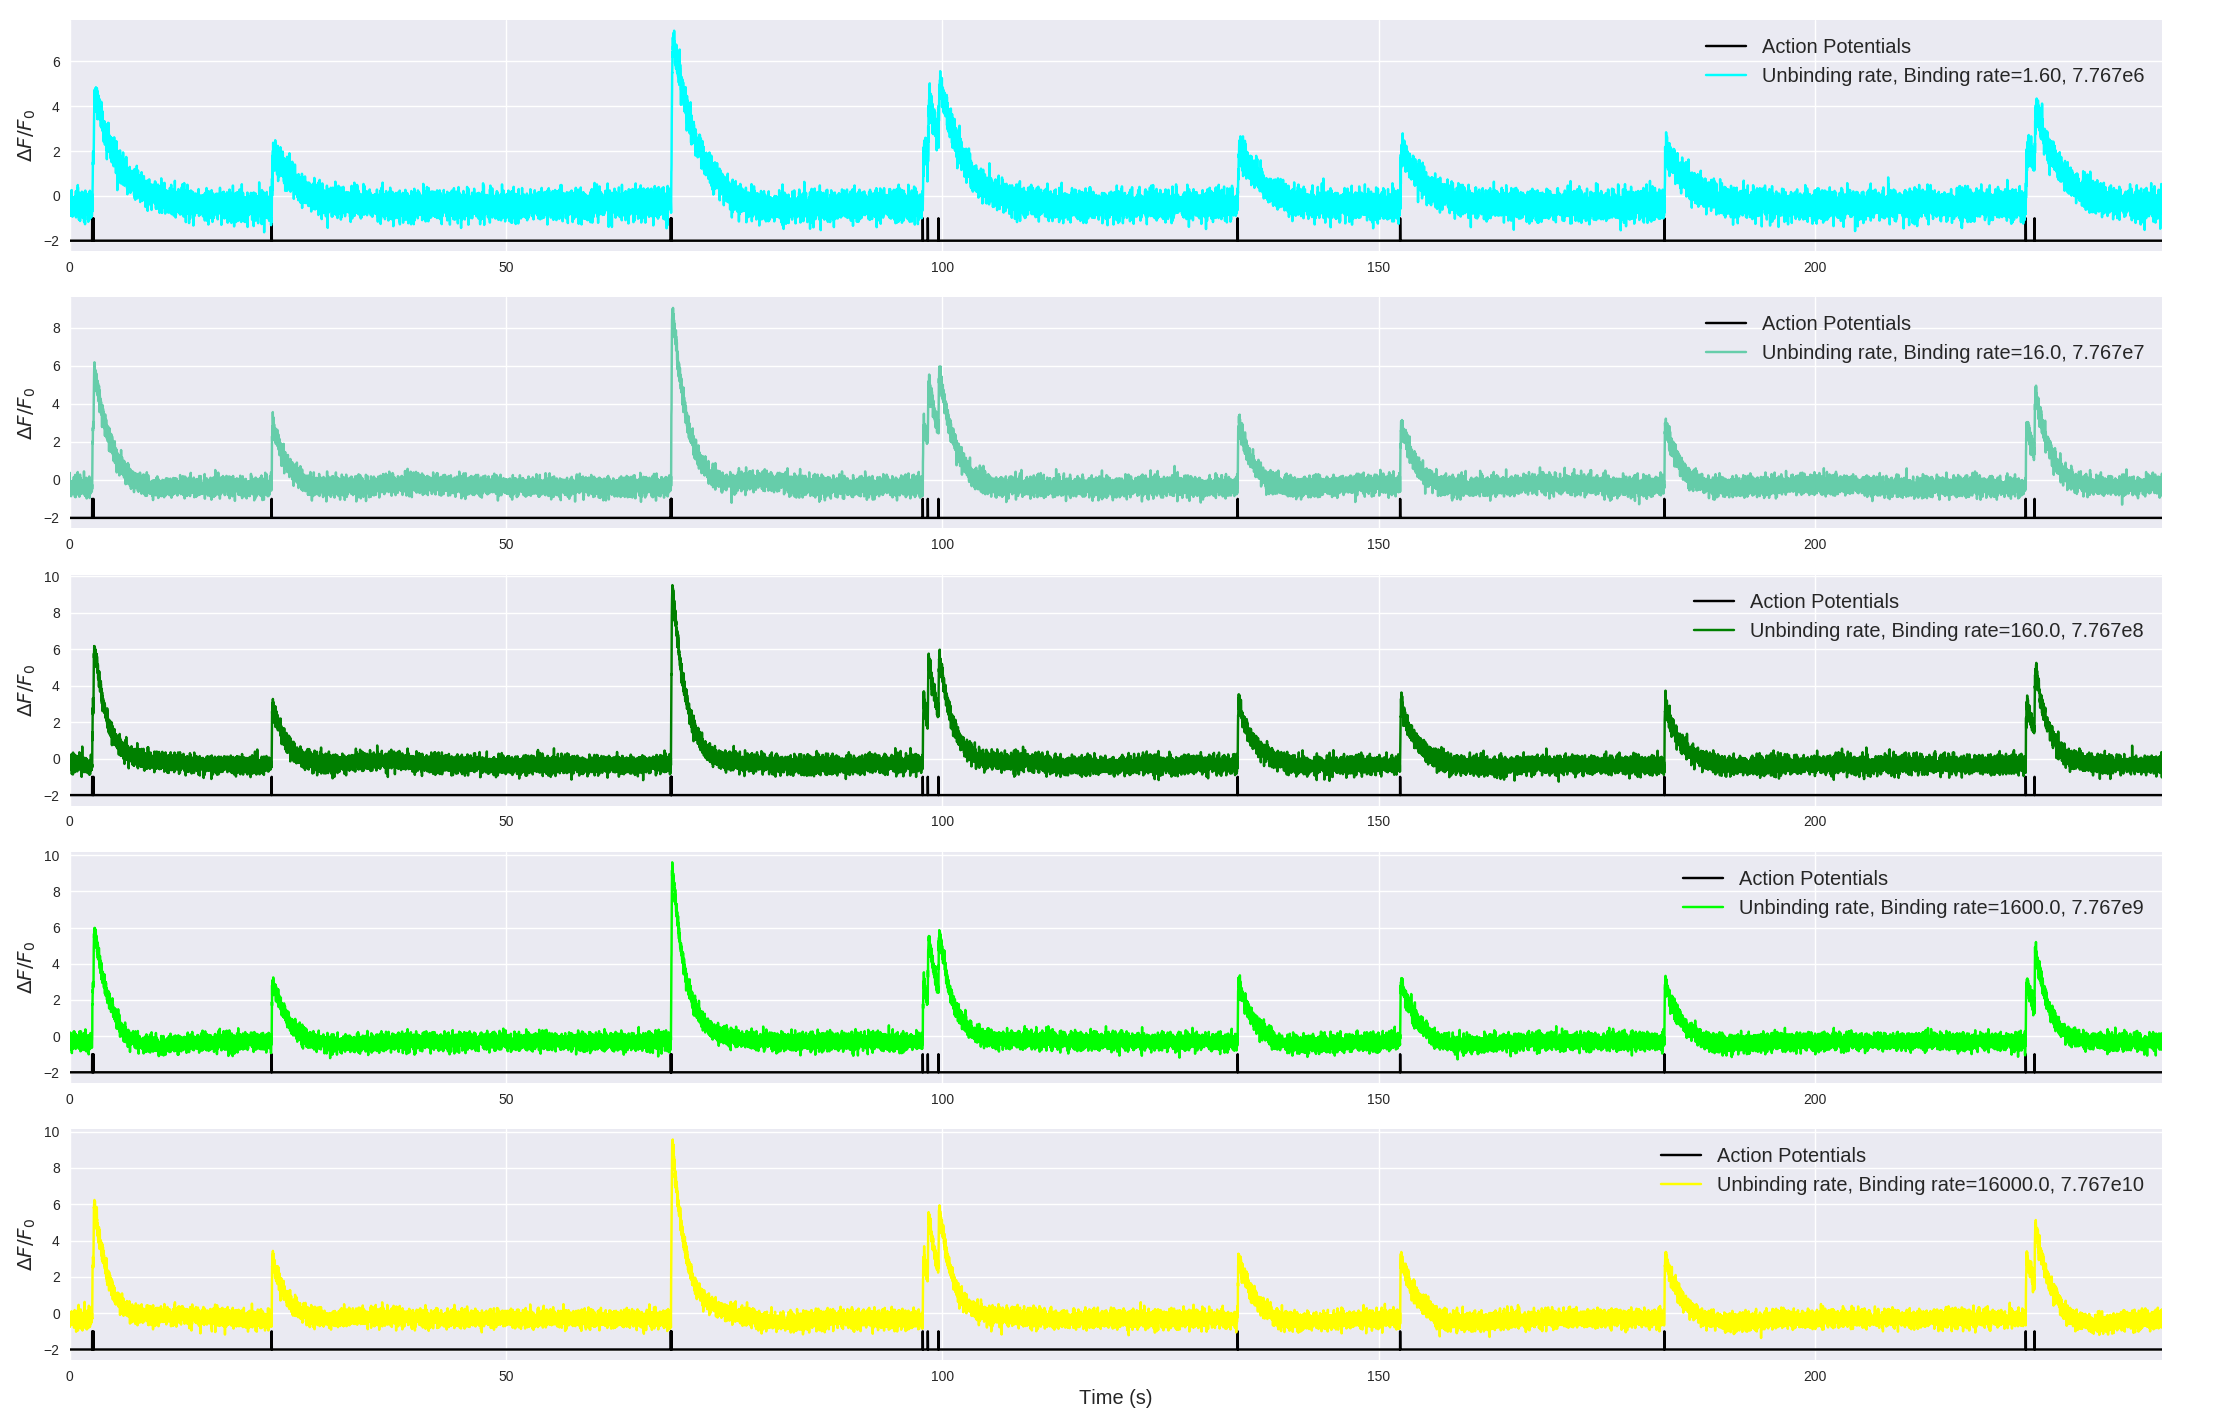
\includegraphics[width=0.33\linewidth]{b_peturbed_fluorescence_18.png}
	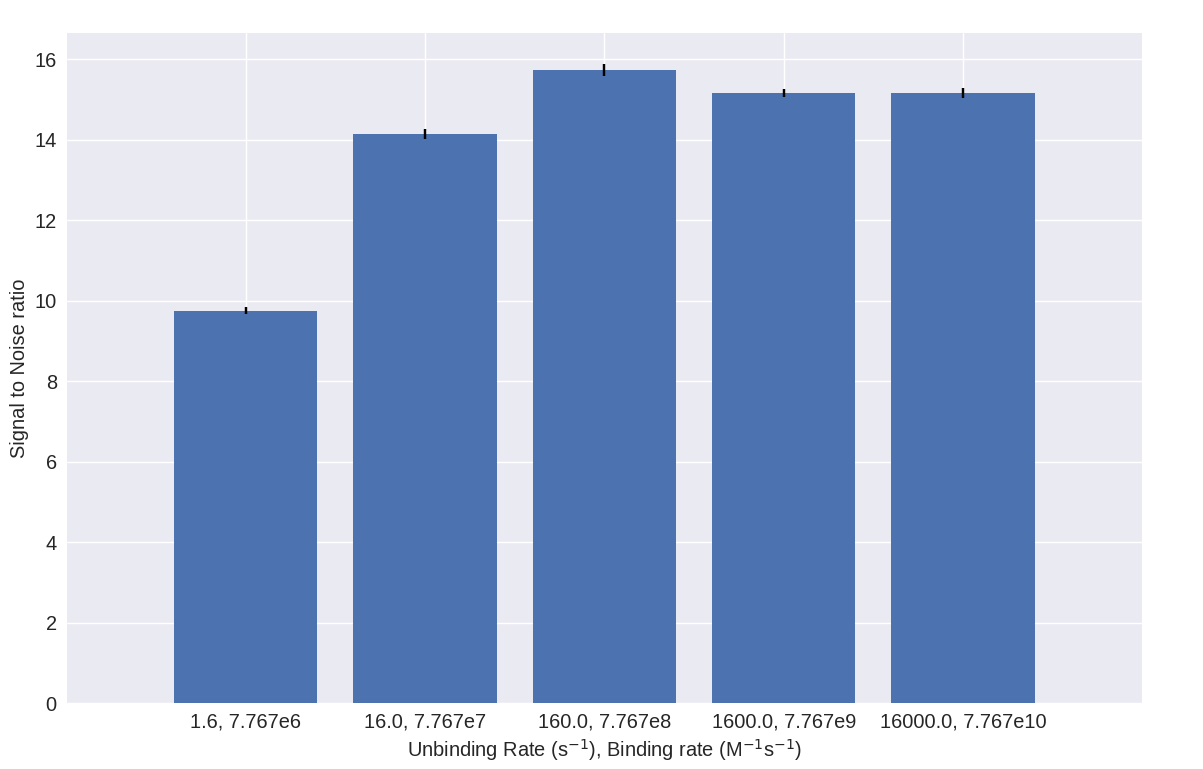
\includegraphics[width=0.33\linewidth]{b_i_f_i_perturbed_snr.png}
	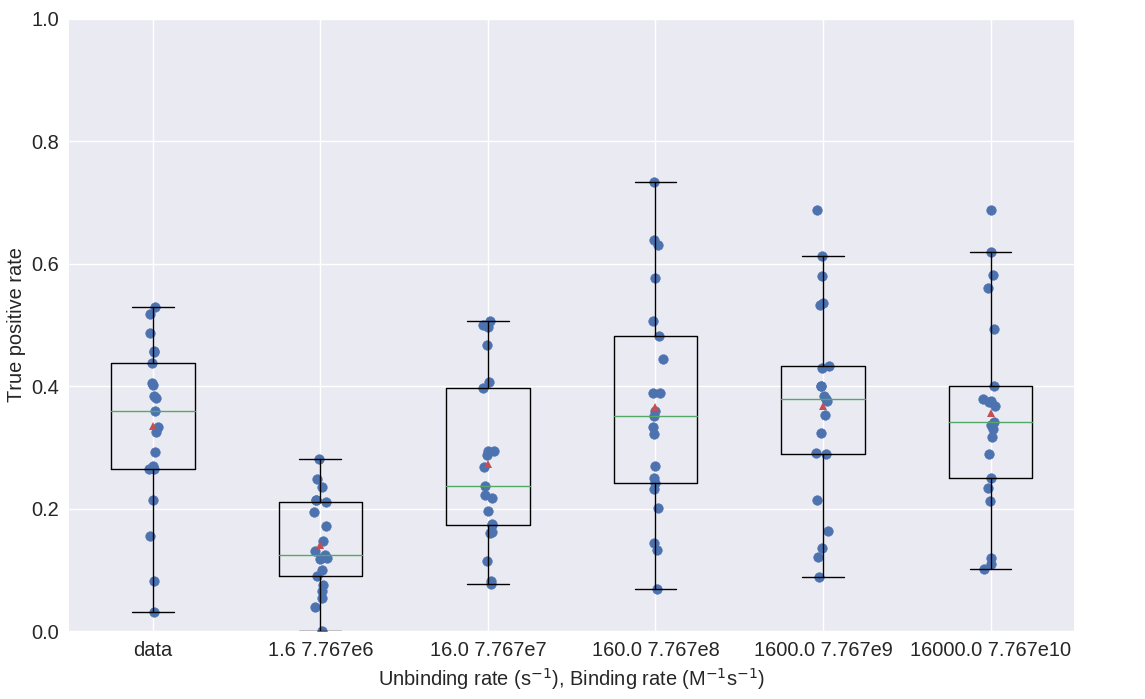
\includegraphics[width=0.33\linewidth]{b_i_f_i_perturbed_oasis_tp.png}
	\caption{(left) An example trace for each of the five pairs of values used for the binding and unbinding rates of the fluorescent calcium indicator.

	(middle) The signal-to-noise ratio of the modelled fluorescence traces using each of the four perturbed values, and the experimental value. The SNRs for the two pairs with values lower than the experimental value are lower than the experimental pair or the higher value pairs.

	(right) The true-positive rates of the deconvolution algorithm's predictions when inferring from the observed data, and inferring from modelled traces using the perturbed and experimental values.}
\end{figure}

\end{block}

\begin{block}{Limitations}
The are a number of limitations to our model. For a start, the equations that define the model do not attempt to model the binding dynamics of calcium buffers such as calmodulin. Specifically, the cooperative or antagonistic pairing between binding sites is not included.

\hspace{2cm} Secondly, there are dozens of different mobile and immobile endogeneous buffers with different association and dissociation rates. Here, we have lumped these buffers together into two modelled concentrations.

\hspace{2cm} Lastly, in this model we have assumed that the indicator bound calcium molecules are constantly under photon bombardment. But in reality, a laser systematically scans across the tissue, exciting molecules as it goes along.

\end{block}

\end{column} % End of the five column

\begin{column}{\sepwid}\end{column} % Empty spacer column

\begin{column}{\onecolwid} % start of column 6

%----------------------------------------------------------------------------------------
%	CONCLUSION
%----------------------------------------------------------------------------------------

\begin{block}{Conclusion}
\begin{itemize}
 	\item We varied the parameters of the model and measured the effect of these variations on the signal to noise ratio of the modelled traces, and the quality of the spike inference. We found that variations in the fluorescent calcium indicator affects the modelled traces, SNR, and spike inference in different ways.

	\item We found that increasing the concentration of immobile endogeneous buffer increased the decay time of the fluorescence traces, decreased the SNR, and decreased the quality of spike inference.

	\item Finally we found that decreasing both the unbinding and binding rates of the fluorescent calcium indicator simultaneously decreases the SNR, and decreases the quality of spike inference.

	\item The parameters of the model can be calibrated to those of different fluorescent indicators, and the any spike train can be used as an input to the model. Therefore, our intention is that this model could be used by researchers to simulate the appearance or characteristics of fluorescence traces under their own specific experimental circumstances. This could help researchers to choose a more suitable indicator, or to assess the challenges associated with using a fluorescent calcium indicator.
\end{itemize}
\end{block}

%----------------------------------------------------------------------------------------
%	ADDITIONAL INFORMATION
%----------------------------------------------------------------------------------------

%\begin{block}{Additional Information}
%
%Spike-finder
%
%Deconvolution algorithm
%
%\end{block}

%----------------------------------------------------------------------------------------
%	REFERENCES
%----------------------------------------------------------------------------------------

\begin{block}{References}

\nocite{*} % Insert publications even if they are not cited in the poster
\small{\bibliographystyle{unsrt}
\bibliography{bna_poster.bbl}}

\end{block}

%----------------------------------------------------------------------------------------
%	ACKNOWLEDGEMENTS
%----------------------------------------------------------------------------------------

\setbeamercolor{block title}{fg=red,bg=white} % Change the block title color

\begin{block}{Acknowledgements}

\small{\rmfamily{I would like to thank Conor Houghton for his help in preparing this poster. This is an EPSRC funded project.}} \\

\end{block}

%----------------------------------------------------------------------------------------
%	CONTACT INFORMATION
%----------------------------------------------------------------------------------------

\setbeamercolor{block alerted title}{fg=black,bg=norange} % Change the alert block title colors
\setbeamercolor{block alerted body}{fg=black,bg=white} % Change the alert block body colors

\begin{alertblock}{Contact Information}

\begin{itemize}
\item Web: \href{http://www.bristol.ac.uk/engineering/research/computational-neuroscience/}{http://www.bristol.ac.uk/engineering/research/computational-neuroscience/}
\item Email: \href{mailto:t.delaney@bristol.ac.uk}{t.delaney@bristol.ac.uk}
\item Address: 	81-83 Woodland Road, \\
								\hspace{3.75cm} University of Bristol, \\
								\hspace{3.75cm} Bristol, \\
								\hspace{3.75cm} BS3 1US, \\
								\hspace{3.75cm} UK
\end{itemize}

\end{alertblock}

\end{column} % end of column 6

\begin{column}{\sepwid}\end{column} % Empty spacer column

\end{columns} % End of all the columns in the poster

\end{frame} % End of the enclosing frame

\end{document}
